\section{Experiments}
\label{sec:experiments}

% In this section, we explore the following key research questions:

% \begin{itemize}[leftmargin=10pt]
%     \item \textbf{RQ1:} : How does RankMixer perform compared with state-of-the-art models in the comparable scale and complexity.
%     \item \textbf{RQ2:} What is the performance scaling curves  when scaling different model structures and which model's scaling law is the most steepest
%     \item \textbf{RQ3:} How does the key commponet in RankMixer affecting its scaling performance
%     \item \textbf{RQ4:} How to analyze and optmize RankMixer model's cost and efficiency in the real-world application.
% \end{itemize}
\subsection{Experiment Settings}

\subsubsection{Datasets and Environment}

The offline experiments were conducted using the training data from the Douyin recommendation system. These data are derived from Douyin's online logs and user feedback labels. The training dataset includes over 300 features, such as numerical features, ID features, cross features, and sequential features, involving billions of user IDs and hundreds of millions of video IDs, which are all converted into embeddings. The data covers trillions of records per day, and experiments were conducted on data collected over a two-week period.

\subsubsection{Evaluation Metrics}

To evaluate model performance, we use AUC (Area Under the Curve) and UAUC (User-level AUC) as the primary performance metrics and Parameter count, FLOPs and MFU as the efficiency metrics listed as follows: \textbf{Finish/Skip AUC/UAUC:} A finish=1/0 or skip=1/0 label indicates whether a user completed watching a video or slide to the next video in a short-time. We evaluate the AUC and UAUC for this finish label. an AUC increase of 0.0001 can be regarded as a confidently significant improvement. \textbf{Dense-Param:} The number of parameters in the dense part, excluding the sparse embedding parameters.  Training \textbf{Flops/Batch:} The number of floating-point operations (FLOPs) required to run a single batch of 512 through the model, representing the computational cost of training.  \textbf{MFU:} MFU(Model FLOPs Utilization) is a metric that measures how effectively a model utilizes floating-point operations provided by the hardware, calculated by dividing the model’s actual FLOPs consumption by the hardware’s theoretical FLOPs capacity.



\subsubsection{Baselines}

We compare against the following widely recognized SOTA baselines: \textbf{DLRM-MLP}:which is the vanilla MLP for feature crossing as the experiment baseline, \textbf{DCNv2}\cite{wang2021dcn},\textbf{RDCN}\cite{DBLP:conf/kdd/BorisyukZSZTPDH24} the Sota of feature cross model. \textbf{MoE} scales up by using mutliply parallel experts. \textbf{AutoInt}\cite{song2019autoint}, \textbf{Hiformer}\cite{gui2023hiformer} combines heterogeneous self-attention layer and low-rank approximation matrix computation. \textbf{DHEN}\cite{zhang2022dhen}: which combines different kind of feature-cross block and stacks multiple layers (DCN/self-attention/FM/LR) \textbf{Wukong}\cite{zhangwukong} investigates the scaling law of feature interaction following the arch of DHEN with Factorization Machine Block (FMB) and Linear Compress Block (LCB).

All experiments were conducted on hundreds of GPUs in a hybrid distributed training framework that the sparse part is updated asynchronously, while the dense part is updated synchronously. The optimizer hyperparameters were kept consistent across all models. For the dense part, we used the RMSProp optimizer with a learning rate of 0.01, while the sparse part used the Adagrad optimizer. 

\subsection{Comparison with SOTA methods}
% 需要在导言区引入:
% \usepackage{graphicx}
% \usepackage{booktabs}

\begin{table}[t]
\centering
\caption{Performance \& efficiency comparison of $\sim$100 M-parameter recommendation models (best values in \textbf{bold}).}
\label{table:main_result}
\resizebox{\linewidth}{!}{%
\renewcommand\arraystretch{1.05}
\begin{tabular}{lcccccc}
\toprule
\multirow{2}{*}{Model} & \multicolumn{2}{c}{\textbf{Finish}} & \multicolumn{2}{c}{\textbf{Skip}} & \multicolumn{2}{c}{\textbf{Efficiency}} \\
\cmidrule(lr){2-3} \cmidrule(lr){4-5} \cmidrule(l){6-7}
 & AUC$\uparrow$ & UAUC$\uparrow$ & AUC$\uparrow$ & UAUC$\uparrow$ & Params & FLOPs/Batch \\
\midrule
DLRM-MLP (base)     & 0.8554 & 0.8270 & 0.8124 & 0.7294 & 8.7 M  & 52 G \\
\midrule
DLRM-MLP-100M       & +0.15\% & —        & +0.15\% & —        & 95 M  & 185 G \\
DCNv2               & +0.13\% & +0.13\% & +0.15\% & +0.26\% & 22 M  & 170 G \\
RDCN                & +0.09\% & +0.12\% & +0.10\% & +0.22\% & 22.6 M & 172 G \\
MoE                 & +0.09\% & +0.12\% & +0.08\% & +0.21\% & 47.6 M & 158 G \\
AutoInt             & +0.10\% & +0.14\% & +0.12\% & +0.23\% & 19.2 M & 307 G \\
DHEN                & +0.18\% & +0.26\% & +0.36\% & +0.52\% & 22 M  & 158 G \\
HiFormer            & +0.48\% & —        & —        & —        & 116 M & 326 G \\
Wukong              & +0.29\% & +0.29\% & +0.49\% & +0.65\% & 122 M & 442 G \\
\midrule
\textbf{RankMixer-100M} & \textbf{+0.64\%} & \textbf{+0.72\%} & \textbf{+0.86\%} & \textbf{+1.33\%} & 107 M & 233 G \\
\textbf{RankMixer-1B}   & \textbf{+0.95\%} & \textbf{+1.22\%} & \textbf{+1.25\%} & \textbf{+1.82\%} & \textbf{1.1 B} & \textbf{2.1T} \\
\bottomrule
\end{tabular}%
}
\end{table}


To explore how to scale up the model, we compare models with similar parameter sizes around 100 million to determine which model structure performs best with the same computational cost.

The main results of the performance of our method and baselines
are summarized in  Table~\ref{table:main_result}.
 We can observe RankMixer significantly outperforms other SOTA models across multiple objectives and metrics.

We take a closer look at each model. First, simply scaling DLRM up to 100 million parameters yields only limited gains, underscoring the necessity of designing models tailored to recommendation data characteristics for better scaling performance. We then compare the RankMixer model with other classic cross-structure designs such as DCN, RDCN, AutoInt, and DHEN, and find they suffer from an imbalance between model parameters and computational cost. Even with relatively small parameter sizes, these models already exhibit large FLOPs, indicating design shortcomings that constrain their results in the table. Meanwhile, although RankMixer achieves the best performance, its FLOPs remain relatively moderate among all the models when scaled to 100 million parameters, reflecting a balanced approach to model capacity and computational load. 

We also compare RankMixer with several commonly used state-of-the-art scaling-up models—like Hiformer and wukong—and find that under similar parameter settings, RankMixer not only performs better but also has lower computational requirements.

\subsection{Scaling Laws of different models}

\begin{figure}
    \centering
    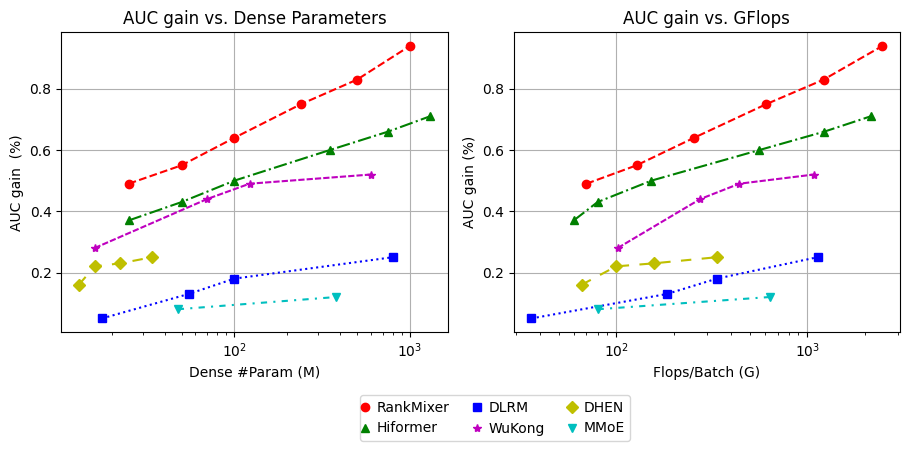
\includegraphics[width=\linewidth]{img/scaling_law.png}
    \caption{Scaling laws between finish Auc-gain and Params/Flops of different models.  The x-axis uses a logarithmic scale.}
    \label{fig:scaling_law}
\end{figure}

In the Figure \ref{fig:scaling_law}, we show the scaling law curves observed from both parameter size and Flops. The RankMixer model shows the steepest scaling law both interms of parameters, and FLOPs. RankMixer is consistently superior to the other models. 

Although the wukong model exhibits a relatively steep parameter curve, its computational cost increases even more rapidly; as a result, the gap between it and both RankMixer and hiformer is even larger on the AUC vs FLOPs curve. Moreover, hiformer’s performance is slightly inferior to RankMixer’s, reflecting that its reliance on token segmentation at a feature level and on Attention affects its efficiency. The scaling of DHEN is not ideal, reflecting the limited scalability of its cross structure. Moreover, MoE’s strategy of scaling by adding experts brings about challenges in maintaining expert balance, which results in suboptimal scaling performance.

To be Sepcific, We can scale up RankMixer model by increasing width ($D$), feature token ($T$) and Layer($L$). In our experiments we observed a conclusion shared with LLM scaling laws: model quality correlates primarily with the total number of parameters, and different scaling directions (depth L, width D, tokens T) yield almost identical performance. From a compute-efficiency standpoint, while larger hidden-dim generate larger matrix-multiply shapes and thus achieve higher MFU than stacking more layers. So the final configuration for 100M and 1B are set as ($D$=768, $T$=16, $L$=2) and ($D$=1536, $T$=32, $L$=2) respectively.

\subsection{Ablation Study}

% We further analyze which specific design factors and structures of the RankMixer model affect its scaling law.


% \subsubsection{Impact of  $D_{\text{input}}$ for Dense scaling}

% \begin{figure}
%     \centering
%     \includegraphics[width=0.6\linewidth]{img/wider_input.png}
%     \caption{Auc-gain Comparison between different $D_{\text{input}}$, $D_{\text{RankMixer}}$ and layers $L$.}
%     \label{fig:wider_input}
% \end{figure}
% The scaling benefits of the upper dense structure are largely constrained by the information available in the input and the base width. If the input becomes a information bottleneck, scaling up the dense parameters will yield limited benefits. Therefore, we increase the $D_{\text{input}}$ from 4000 dimensions to 15000 dimensions with scaling up the size of sparse embeddings and $e_h$ from  . As shown in Figure \ref{fig:wider_input}, the scaling law becomes more pronounced when the input is expanded, removing the input bottleneck.
    
% \begin{table}[h]
%     \centering
%     \caption{Ablation Study Results based on the modification of RankMixer-100M}
%     \resizebox{0.4\textwidth}{!}{%
%     \begin{tabular}{c|c}
%         \hline
%         Setting & AUC Diff \\
%         \hline
%         w\textbackslash{}o skip Connections & -0.07\% \\
%         w\textbackslash{}o Multi-head Token Mixing & -0.50\% \\
%         w\textbackslash{}o LayerNorm & -0.05\% \\
%         replace Per-Token FFN with all-shared FFN & -0.31\% \\
%         \hline
%         \hline
%         token-routing strategy comparison & \textbackslash{}N \\
%         \hline
%         All-Concat-MLP & -0.18\% \\
%         All-Share & -0.25\% \\
%         Self-Attention & -0.03\% \\        
%         \hline
%     \end{tabular}
%     }
%     \label{ablation study}
% \end{table}

\begin{table}[h]
\centering
\caption{Ablation on components of RankMixer-100M}
\label{ablation study}
\small
\begin{tabular}{@{\quad}l c@{\quad}}
\toprule
\textbf{Setting} & $\Delta$AUC \\ 
\midrule
w/o skip connections                          & $-0.07\%$ \\
w/o multi-head token mixing                   & $-0.50\%$ \\
w/o layer normalization                       & $-0.05\%$ \\
Per-token FFN $\rightarrow$ shared FFN        & $-0.31\%$ \\
\bottomrule
\end{tabular}
\end{table}

%-------------------------------------------------------
% Table 2 – routing–strategy comparison
\begin{table}[h]
\centering
\caption{Token2FFN Routing–strategy comparison}
\label{ablation-routing}
\small
\begin{tabular}{@{\quad}l c c c@{\quad}}
\toprule
\textbf{Routing strategy} & $\Delta$AUC & $\Delta$Params & $\Delta$FLOPs \\ 
\midrule
All-Concat-MLP & $-0.18\%$ & 0.0\% & 0.0\% \\
All-Share      & $-0.25\%$ & 0.0\% & 0.0\% \\
Self-Attention & $-0.03\%$ & +16\% & +71.8\% \\
\bottomrule
\end{tabular}
\end{table}

In the RankMixer-100M model, we performed ablation studies on residual connections, Multi-Head Token-Mixing. From Table \ref{ablation study}, we can see that removing these components significantly decreased the model's performance. Removing Multi-Head Token-Mixing loses global information, as each FFN only models partial features without interaction. Removing residual connections and LayerNorm also worsens performance, reducing training stability and making gradient explosion or vanishing issues more likely.
% 
\begin{table*}[h]
\caption{Online AB test result for Feed Recommendation Scenarios in both Douyin and Douyin lite app and the improvements are all statistically significant. According to long-term reverse A/B tests and continuous observations over long-term reverse experiments, the gains provided by RankMixer-1B have not yet converged, and the results presented here are still improving.}
\resizebox{\textwidth}{!}{
\renewcommand\arraystretch{1.08}
\begin{tabular}{lcccclccccl}
\hline
                       & \multicolumn{5}{c}{\textbf{Douyin app}}                                                      & \multicolumn{4}{c}{\textbf{Douyin lite}}                                  &                  \\ \cmidrule(lr){2-6}\cmidrule{7-11} 
                       & \textbf{Active Day}$\uparrow$ & \textbf{Duration}$\uparrow$ & \textbf{Like}$\uparrow$ & \textbf{Finish}$\uparrow$ & \textbf{Comment}$\uparrow$ & \textbf{Active Day}$\uparrow$ & \textbf{Duration}$\uparrow$ & \textbf{Like}$\uparrow$ & \textbf{Finish}$\uparrow$ & \textbf{Comment}$\uparrow$ \\ \hline

\textbf{Overall}       & +0.2908\%           & +1.0836\%         & +2.3852\%     & +1.9874\%       & +0.7886\%        & +0.1968\%           & +0.9869\%          & +1.1318\%     & +2.0744\%        & +1.1338\%        \\ \hline 
\textbf{Low-active}    & +1.7412\%            & +3.6434\%         & 
+8.1641\%     & +4.5393\%       & +2.9368\%         & +0.5389\%           & +2.1831\%         & +4.4486\%      & +3.3958\%       & +0.9595\%        \\
\textbf{Middle-active} & +0.7081\%           & +1.5269\%         & +2.5823\%     & +2.5062\%       & +1.2266\%         & +0.4235\%           & +1.9011\%         & +1.7491\%      & +2.6568\%         & +0.6782\%        \\
\textbf{High-active}   & +0.1445\%           & +0.6259\%         & +1.828\%      & +1.4939\%       & +0.4151\%          & +0.0929\%           & +1.1356\%         & +1.8212\%      & +1.7683\%        & +2.3683\% 
\\ \hline
\end{tabular}
}
\label{online_ab}
\end{table*}

\begin{table}[t]
\centering
\caption{Online lift of RankMixer in Advertising}
\label{tab:ads-search}
% \resizebox{0.9\linewidth}{!}{%
\footnotesize
\renewcommand\arraystretch{0.95}
\begin{tabular}{@{}lccc@{}}
\toprule
 & \multicolumn{2}{c}{\textbf{Advertising}}\\
\cmidrule(lr){2-3}
Metric & $\Delta$AUC$\uparrow$ & ADVV$\uparrow$  \\
\midrule
Lift  & +0.73\% & +3.90\%\\
\bottomrule
\end{tabular}%
\label{ad_search}
\end{table}
% \begin{table}[h]
%     \centering
%     \caption{Token Routing Strategies}
%     \begin{tabular}{|c|c|c|}
%         \hline
%         Strategy & AUC & Flops \\
%         \hline
%         All-Concat-MLP & 0.XX & X \\
%         Self-Attention & 0.XX & X \\
%         All-Share & 0.XX & X \\
%         Multi-Head Token-Mixing & 0.XX & X \\
%         \hline
%     \end{tabular}
% \end{table}
        
We further analyzed the token mixing strategies, i.e., the routing strategies from feature tokens to FFNs in the Table \ref{ablation-routing}. The routing strategies compared with Multi-Head Token Mixing (Multi-Head Token-Mixing) include: \textit{All-Concat-MLP:} Concatenates all tokens and processes them through a large MLP before splitting them into the same number of tokens. The decrease of performance shows the challenges in learning large matrices and weakening local information learning. \textit{All-Share:} No splitting, the entire input vector is shared and fed to each per-token FFN similar as MoE. The performane declines siginifantly which show the importance of feature subspace split and independent modeling contrast to all-shared input.
\textit{Self-Attention:} Applies self-attention between tokens for routing. Its performance is slightly inferior to the Multi-Head Token-Mixing and also suffers from high computational cost, which shows the difficulty of learning similarity across hundreds of different feature subspaces. 

\subsection{Sparse-MoE Scalability and Expert Balance}
\label{sec:smr_results}

\begin{figure}
    \centering
    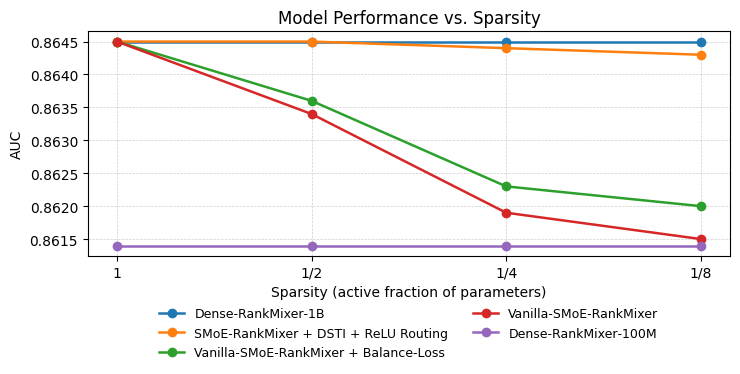
\includegraphics[width=\linewidth]{img/MoE.png}
    \caption{AUC performance of RankMixer variants under decreasingly sparse activation ratio (1,1/2,1/4,1/8 of experts): dense-training + ReLU-routed SMoE preserves almost all accuracy of the 1 B dense model.}
    \label{fig:sparsity_curve}
\end{figure}

\paragraph{Scalability.}
Figure~\ref{fig:sparsity_curve} plots offline \textsc{AUC} gains versus Sparsity of SMoE. Combining Dense-Training-Sparse-Inference with ReLU routing is essential for preserving accuracy under aggressive sparsity, enabling RankMixer to scale parameter capacity (and memory footprint) by > 8× with nearly no loss in AUC and with substantial inference-time savings (+50\% improvement over throughput).  Vanilla SMoE's performance drops monotonically as fewer experts are activated, illustrating the expert-imbalance and under-training issues we identified. Adding a load-balancing loss reduces the degradation relative to vanilla SMoE, yet still falls short of the DTSI + ReLU version because the problems mostly lies in the expert training instead of the router.
This validates Sparse-MoE as the
path to scale RankMixer from the current 1\,B parameters to future
10\,B-scale deployments without breaching the cost budgets.


\begin{figure}
    \centering
    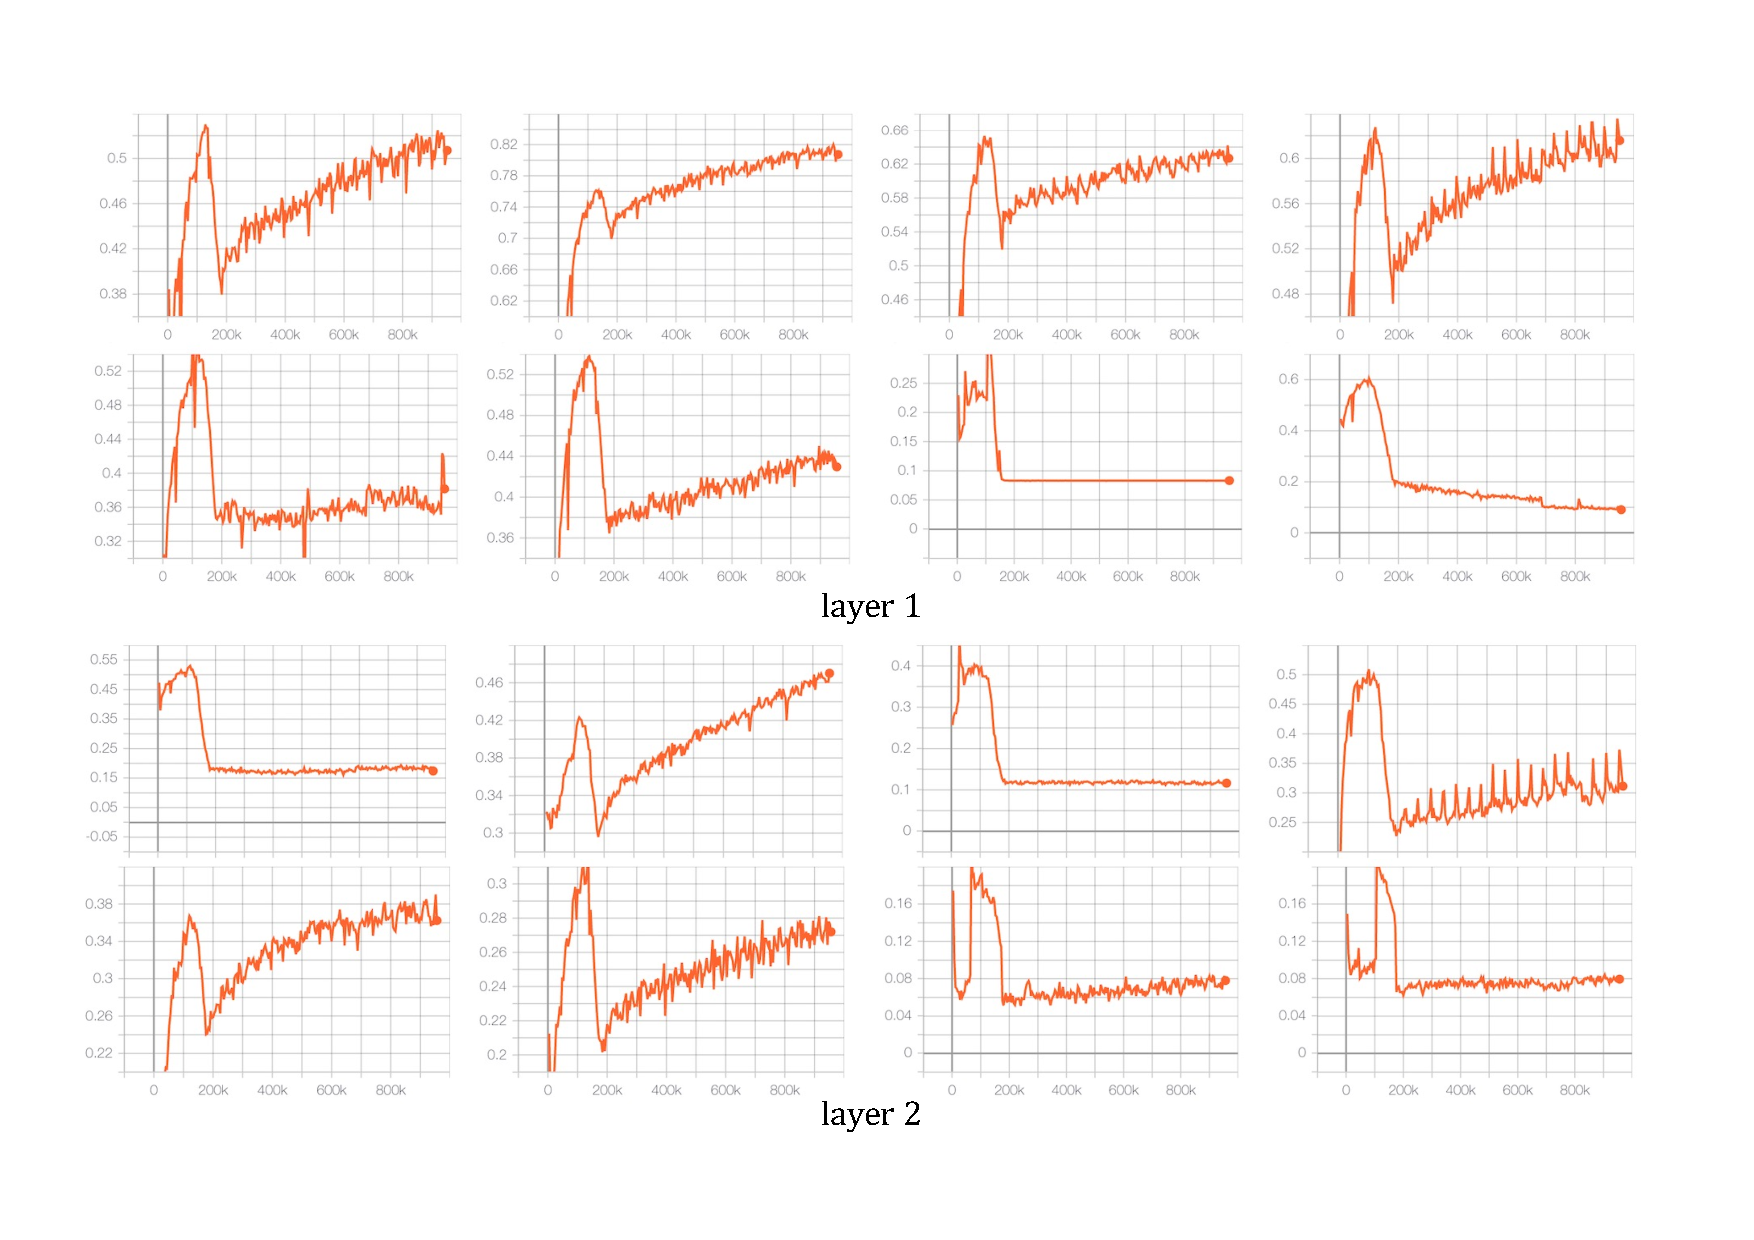
\includegraphics[width=0.7\linewidth]{img/expert_balance.pdf}
    \caption{activated expert ratio for different {\text{token}} in {\text{RankMixer}}.}
    \label{fig:expert_balance}
\end{figure}


\begin{table*}[h]
\caption{Online AB test result for Feed Recommendation Scenarios in both Douyin and Douyin lite app and the improvements are all statistically significant. According to long-term reverse A/B tests and continuous observations over long-term reverse experiments, the gains provided by RankMixer-1B have not yet converged, and the results presented here are still improving.}
\resizebox{\textwidth}{!}{
\renewcommand\arraystretch{1.08}
\begin{tabular}{lcccclccccl}
\hline
                       & \multicolumn{5}{c}{\textbf{Douyin app}}                                                      & \multicolumn{4}{c}{\textbf{Douyin lite}}                                  &                  \\ \cmidrule(lr){2-6}\cmidrule{7-11} 
                       & \textbf{Active Day}$\uparrow$ & \textbf{Duration}$\uparrow$ & \textbf{Like}$\uparrow$ & \textbf{Finish}$\uparrow$ & \textbf{Comment}$\uparrow$ & \textbf{Active Day}$\uparrow$ & \textbf{Duration}$\uparrow$ & \textbf{Like}$\uparrow$ & \textbf{Finish}$\uparrow$ & \textbf{Comment}$\uparrow$ \\ \hline

\textbf{Overall}       & +0.2908\%           & +1.0836\%         & +2.3852\%     & +1.9874\%       & +0.7886\%        & +0.1968\%           & +0.9869\%          & +1.1318\%     & +2.0744\%        & +1.1338\%        \\ \hline 
\textbf{Low-active}    & +1.7412\%            & +3.6434\%         & 
+8.1641\%     & +4.5393\%       & +2.9368\%         & +0.5389\%           & +2.1831\%         & +4.4486\%      & +3.3958\%       & +0.9595\%        \\
\textbf{Middle-active} & +0.7081\%           & +1.5269\%         & +2.5823\%     & +2.5062\%       & +1.2266\%         & +0.4235\%           & +1.9011\%         & +1.7491\%      & +2.6568\%         & +0.6782\%        \\
\textbf{High-active}   & +0.1445\%           & +0.6259\%         & +1.828\%      & +1.4939\%       & +0.4151\%          & +0.0929\%           & +1.1356\%         & +1.8212\%      & +1.7683\%        & +2.3683\% 
\\ \hline
\end{tabular}
}
\label{online_ab}
\end{table*}

\begin{table}[t]
\centering
\caption{Online lift of RankMixer in Advertising}
\label{tab:ads-search}
% \resizebox{0.9\linewidth}{!}{%
\footnotesize
\renewcommand\arraystretch{0.95}
\begin{tabular}{@{}lccc@{}}
\toprule
 & \multicolumn{2}{c}{\textbf{Advertising}}\\
\cmidrule(lr){2-3}
Metric & $\Delta$AUC$\uparrow$ & ADVV$\uparrow$  \\
\midrule
Lift  & +0.73\% & +3.90\%\\
\bottomrule
\end{tabular}%
\label{ad_search}
\end{table}

\begin{table}[h]
    \caption{Metrics of Online Model Deployment and Cost}
    \resizebox{0.48\textwidth}{!}{%
    \begin{tabular}{c|c|c|c}
        \hline
        Metric & OnlineBase-16M & RankMixer-1B & Change \\
        \hline
        \#Param & 15.8M & 1.1B & $\uparrow$ \textbf{70$\times$} \\
        FLOPs & 107G & 2106G & $\uparrow$ 20.7$\times$ \\
        Flops/Param(G/M) & 6.8 & 1.9 & $\downarrow$ 3.6$\times$ \\
        MFU & 4.47\% & \textbf{44.57}\% & $\uparrow$ 10$\times$ \\
        Hardware FLOPs & fp32 & fp16 & $\uparrow$ 2$\times$ \\
        Latency & 14.5ms & \textbf{14.3ms} & - \\
        \hline
    \end{tabular}%
    }
    \label{case_study}
\end{table}


\paragraph{Expert balance and diversity.}
Vanilla Sparse MoE often suffers from expert imbalance, which in turn leaves some experts under-trained and eventually leads to “dying experts” (experts that are almost never activated) and only a few fixed experts are constantly activated.
Figure~\ref{fig:expert_balance} shows that combining DTSI (dense-training, sparse-inference) with ReLU routing effectively resolves this issue: Dense-training guarantees that most expert receives sufficient gradient updates, preventing expert starvation.
ReLU routing makes the activation ratio dynamic across tokens—the activation proportion shows in the figure varies adaptively according to its information content, which aligns well with the diverse and highly dynamic distribution of recommendation data.
\subsection{Online Serving cost}


How can we prevent inference latency from exploding with a two-order-of-magnitude increase in parameters? In practical systems, latency is inversely proportional to throughput and directly proportional to the cost of serving machine resources. 
Compared to our previous fully-deployed 16M-parameter model (with a structure integrated with DLRM and DCN), our RankMixer model scaled parameters by approximately 70$\times$ to 1B. Despite this significant parameter increase, the final inference latency remained stable due to our hardware-aligned model design and optimization strategies.

When greatly increasing model parameters, latency can be decomposed into the following formula:
\[
\text{Latency} = \frac{\#\text{Param} \times \text{FLOPs/Param ratio}}{\text{MFU} \times \text{(Theoretical Hardware FLOPs)}}
\]
As illustrated in Table~6, the two-order-of-magnitude parameter increase is progressively counteracted by \textbf{3.6$\times$} decrease of FLOPs/Param ratio, \textbf{10\,$\times$} increase of MFU and Quatization-based \textbf{2\,$\times$} Hardware FlOPs improvements.

% 在线上实际部署对比我们在线全量的一个16M的模型（一个融合了DLRM和DCN 结构），我们1B的模型在参数量上提升了约70倍到1B，但通过hardware-aligned model design和优化，最终latency持平。

% 当大幅提升模型参数后，latency可以breakdown成以下公式
% latency = \frac{#Param * FLOPs/Param ratio} {MFU * (机器理论算力)}。
% 从表格6中可以看到，两个数量级的参数increase是如何被逐步拆解抵消的。
\begin{enumerate}[leftmargin=1.3em]
    \item \textbf{FLOPs/Param ratio.}  
          The three row of Table~\ref{case_study} reports the number of floating-point operations (FLOPs) required \emph{per parameter}.  
          Thanks to the model design, RankMixer achieves a 70-fold increase in parameters with only around a 20-fold increase in FLOPs, achieving only one-third the FLOPs/Param ratio of the baseline—a \textbf{3.6,$\times$ efficiency gain}. In other words, RankMixer can accommodate three times more parameters than the baseline at the same FLOPs budget.
    \item \textbf{Model FLOPs Utilization (MFU).}  
          Also shown in Table~\ref{case_study}, MFU indicates the utilization of machine computing.  
          By using large GEMM shapes, good parallel topology (fusing parallel per-token FFNs into one kernel), reduce the memory bandwith cost and overhead, RankMixer raises MFU by nearly \textbf{10\,$\times$}, shifting the model from an \textit{Memory-bound} to a \textit{Compute-bound} regime.
    \item \textbf{Quantization}
         Half-precision (fp16) inference will increase the theoretical peak Hardware FLOPS of GPUs by \textbf{2\,$\times$}.The primary computations in RankMixer consist of several large matrix multiplications that are well suited for half-precision (fp16) inference as mentioned before
\end{enumerate}



\subsection{Online Performance }
To verify the universality of RankMixer as a scaling
recommendation model framework, we conducted online experiments in the two
core application scenarios of personalised ranking—\emph{feed
recommendation} and \emph{advertising}, covering
major use-cases of personalized ranking.
For each scenario we monitor the following key performance indicators:
\begin{itemize}
  \item \textbf{Feed–Recommendation.}  
        \emph{Active Days} is he average number of active days per user during the experiment period, a substitute for DAU growth.;  
        \emph{Duration} measures cumulative stay time on the App;  
        \emph{Finish/Like/Comment:} User's total complete plays, likes, and comments.
  \item \textbf{Advertising.}  
        We report the model quality metrics ($\Delta\emph{AUC}$) and revenue metrics
         \emph{ADVV} (Advertiser Value).
  % \item \textbf{Search.}  
  %       Quality is gauged by query-level $\Delta\emph{AUC}$,
  %       \emph{Active Days}, and \emph{Query-change rate} which measures how often users modify their initial search queries during a search session and lower is better;.
\end{itemize}

% \begin{itemize}[leftmargin=10pt]
%     \item \textbf{Active Days:} The average number of active days per user during the experiment period, a substitute for DAU growth.
%     \item \textbf{Duration:} The total time user spend on the app.
%     \item \textbf{Finish/Like/Comment:} User's number of complete plays, likes, and comments.
% \end{itemize}

% \begin{figure}
%     \centering
%     \includegraphics[draft,width=0.8\linewidth]{img/wider_input.png}
%     \caption{Online A/B test: the AAD improvement across days}
%     \label{fig:scale_dim}
% \end{figure}
The Previous baselines in these scenarios are 16M parameter model combined with DLRM and DCN. We replaced the Dense part with the RankMixer-1B model improving a 0.7\% AUC. We conduct online A/B test experiments across Feed Recommendation and Advertising. The long-term observation of A/B test result on Feed Recommendation for 8 months  are shown on the Table \ref{online_ab} \footnote{This result was updated on July 24, 2025, since the long-term experiments indicating the gains had not yet saturated.}
\unskip and the result of Advertising is shown on the Table \ref{ad_search}.

% The online results show significant improvements in Active Days, Duration, and finish, like rate across multiple activeness user groups.

RankMixer was deployed and evaluated in the three personalised-ranking application including the Feed Recommendation (RankMixer-1B) and Advertising (RankMixer-1B). RankMixer delivered statistically significant uplifts on all business-critical metrics. We can also observe that the improvements on low-active users are largest on the Table \ref{online_ab} compared to other activeness level user groups with over 1.7412\% Active Days improvements, which demonstrates the model’s strong generalization capability.
These results demonstrate that the RankMixer as a unified backbone generalises reliably to different application scenarios. 





